\documentclass{../exhibit}

\title{Look at me Gems}

%% Font
\usepackage{imfellEnglish}
\usepackage[T1]{fontenc}
\raggedright

\usepackage{background}

\backgroundsetup{
scale=1,
color=black,
opacity=0.4,
angle=0,
contents={%
  \includegraphics[height=\paperheight]{mapBackground.jpg}%%https://upload.wikimedia.org/wikipedia/commons/8/81/Nautical_chart_of_the_West_Indies_1797.jpg
  }%
}




%% For the context
%% https://tex.stackexchange.com/questions/86150/torn-page-effect/86151#86151
\usepackage{tikz}
\usetikzlibrary{decorations.pathmorphing}
\definecolor{paper}{RGB}{239,227,157}





\renewcommand{\maketitle}{ %
  \begin{center}
    \scalebox{8}{\thetitle}
  \end{center}
  
\begin{tabular*}{\textwidth}{c @{\extracolsep{\fill}} c}  
\resizebox{4in}{!}{\begin{minipage}[b]{3in}\huge\directions\end{minipage}} &
  \resizebox{4in}{!}{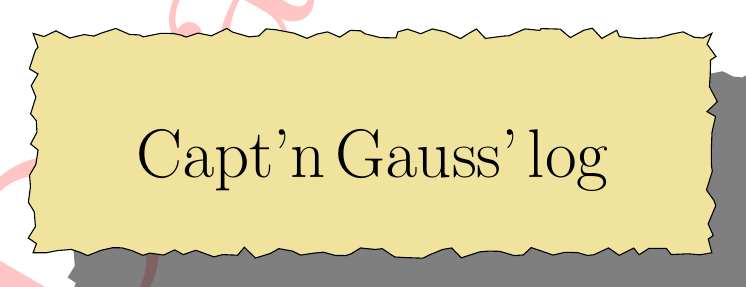
\begin{tikzpicture}[pencildraw/.style={ %
    decorate,
    decoration={random steps,segment length=4pt,amplitude=2pt}
    } %
]
\node[
preaction={fill=black,opacity=.5,transform canvas={xshift=.5cm,yshift=-.5cm}},
pencildraw,draw,fill=paper,text width=3in,inner sep=.5cm] 
{\begin{center}\Huge Capt'n Gauss' log \end{center}\vspace{.7cm} {\huge\context}};
\end{tikzpicture}}

\end{tabular*}

\vfill

\includegraphics[width=3in]{logoPirate.png}\hfill \includegraphics[width=2in]{bammLogo.png}


}


\begin{document}


\begin{context}
  Arr, Capt'n Euler be known fer his ability to discover hidden gems.


  In this here task, ye need to be countin'
  \begin{itemize}
  \item the number o' corners, $C$
  \item number o' edges, $E$
  \item and number o' faces, $F$
  
  \end{itemize}
  on me GEMS!



  Capt'n Euler's characteristic be:
  \[
  C - E + F
  \]
  and it be the biggest GEM of them all!
\end{context}


\begin{directions}
  For each polyhedron,
  \begin{itemize}
  \item count the number of \\ Corners
  \item count the number of \\ Edges
  \item and count the number of \\ flat Faces 
  
  \end{itemize}
  Compute:


  Corners - Edges + Faces
\end{directions}



\begin{example}

  Me cubical sapphire has $8$ Corners, $12$ Edges, and $6$ Faces.
  \begin{center}
\raisebox{-1.5in}{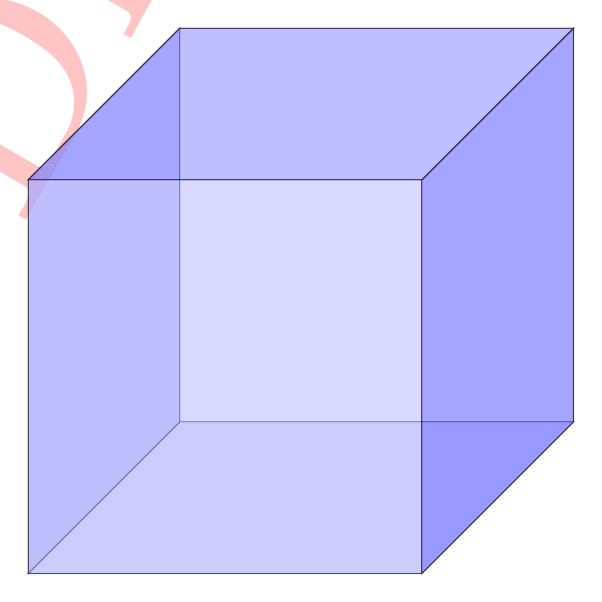
\begin{tikzpicture}[scale=5]
\draw[fill=blue!40,opacity=0.5] (0,0,0) -- (1,0,0) -- (1,0,1) -- (0,0,1) -- cycle;
\draw[fill=blue!20,opacity=0.5]  (0,0,0) -- (0,1,0) -- (1,1,0) -- (1,0,0) -- cycle;
\draw[fill=blue!60,opacity=0.5]  (0,0,0) -- (0,0,1) -- (0,1,1) -- (0,1,0) -- cycle;
\draw[fill=blue!20,opacity=0.5]  (0,0,1) -- (0,1,1) -- (1,1,1) -- (1,0,1) -- cycle;
\draw[fill=blue!60,opacity=0.5]  (1,0,0) -- (1,0,1) -- (1,1,1) -- (1,1,0) -- cycle;
\draw[fill=blue!40,opacity=0.5]  (0,1,0) -- (1,1,0) -- (1,1,1) -- (0,1,1) -- cycle;
\end{tikzpicture}}
\qquad C - E + F = 2
  \end{center}
\end{example}



\begin{mathConnections}
  https://bartsnapp.github.io/Math-Outreach-Exhibits/eulerCharacteristic/
\end{mathConnections}
\end{document}
